\newcommand{\env}[1]{\texttt{#1}}
\newcommand{\command}[1]{\texttt{#1}}
\newcommand{\package}[1]{\texttt{\itshape#1}}
\newcommand{\engl}[1]{(engl: \textit{#1})\xspace}
\setlength{\parindent}{0pt}
\newpage

\section{Aufgabe 1}\cite{[1,2]}

\subsection{Frage- bzw. Aufgabenstellung}

Sie sollen ein Chat-System unter Verwendung von Java RMI implementieren. Das System besteht aus einem Server, an den beliebig viele Clients angeschlossen werden können. Das System soll nach bekanntem Prinzip arbeiten: Nachrichten werden auf einem Client eingegeben und über den Server an alle angeschlossenen Clients weiter geleitet.

\subsection{Lösung}

Zunächst wurden die Interfaces für das ChatSystem realisiert. Eins wurde \textit{ChatServerIF} genannt (siehe Zeile 1 bis 8), und das andere \textit{ClientProxyIF} (siehe nächstes Listing, Zeile 1 bis 4).

\begin{lstlisting}
public interface ChatServerIF extends Remote {
	public void subscribeUser (ClientProxyIF handle) throws RemoteException;
	
	public boolean unsubscribeUser (ClientProxyIF handle) throws RemoteException;
	
	public void broadcast(String message) throws RemoteException;
	
}
\end{lstlisting}

\begin{lstlisting}
public interface ClientProxyIF extends Remote {
	public void receiveMessage (String message) throws RemoteException;
	
}
\end{lstlisting}


Danach wurde eine Klasse \textit{ChatServerImpl} realisiert, die das Interface ChatServerIF implementiert. Hierzu wurde eine neue List \textit{clients} deklariert, die Objekte von \textit{ClientProxyIF} beinhalten kann. Diese List wird dann im Konstruktor der Klasse instanziiert (siehe Zeile 1 bis 11). Wichtig für diese, wie auch für die \textit{ChatClient} Klasse ist, dass beide Klassen von \textit{UnicastRemoteObject} erben, damit man Remote-Objects exportieren kann.

\begin{lstlisting}
public class ChatServerImpl extends UnicastRemoteObject implements ChatServerIF {

	/**
	 * 
	 */
	private static final long serialVersionUID = 1L;
	private List<ClientProxyIF> clients;

	public ChatServerImpl() throws RemoteException {
		this.clients = new ArrayList<ClientProxyIF>();
	}
\end{lstlisting}


Für die Methoden um einen neuen User zu erstellen oder einen vorhandenen User zu löschen, wurden nun die Methoden aus dem Interface \textit{ChatServerIF} implementiert. Die Methode \textit{subscribeUser} bekommt als Parameter ein Objekt vom Typ \textit{ClientProxyIF} und fügt der List \textit{clients} einfach das übergebene Objekt hinzu. Bei der Methode \textit{unsubscribeUser} funktioniert dies so ähnlich, nur das hier logischerweise das ClientProxyIF-Objekt aus der List entfernt wird (siehe Zeile 1 bis 9).

\begin{lstlisting}
	@Override
	public void subscribeUser(ClientProxyIF handle) throws RemoteException {
		this.clients.add(handle);
	}

	@Override
	public boolean unsubscribeUser(ClientProxyIF handle) throws RemoteException {
		return this.clients.remove(handle);
	}
\end{lstlisting}


Schließlich wird noch die Methode \textit{broadcast} implementiert, die dafür sorgt, dass jeder Client die eingegebene Nachricht bekommt. Hierfür wird mit einer for-Schleife die komplette clients-List iteriert, wobei jeder Client dann mithilfe der \textit{receiveMessage-Methode} diese Nachricht empfängt (siehe Zeile 1 bis 8). Auf die receiveMessage-Methode wird noch später eingegangen.

\begin{lstlisting}
	@Override
	public void broadcast(String message) throws RemoteException {
		for (int i = 0; i < clients.size(); i++) {
			clients.get(i).receiveMessage(message);
		}

	}
\end{lstlisting}	


Zuletzt wird noch die \textit{main} erzeugt, in der eine Referenz auf ein entferntes Objekt gespeichert wird. Dies wird mit der Klasse \textit{Naming} und der Methode \textit{rebind} erreicht (siehe Zeile 1 bis 5). Als Parameter werden ein Name und ein neues Objekt angegeben.

\begin{lstlisting}
	public static void main(String[] args) throws RemoteException, MalformedURLException {
		Naming.rebind("RMIChatServer", new ChatServerImpl());
	}

}
\end{lstlisting}

Jetzt wird die \textit{ChatClient} Klasse erstellt, die das Interface \textit{ClientProxyIF} und \textit{Runnable} implementiert, da die run-Methode überschrieben werden muss. \\
\\
Die Klasse bekommt ein Objekt \textit{chatServer} vom Typ ChatServerIF, welches dann am Ende, wie der Name schon sagt, den Server darstellen soll. Dann wird noch ein String name erstellt, der den Namen des Clients darstellt und es wird noch ein boolean gebraucht, welcher in der überschriebenen run-Methode zum Einsatz kommt (siehe Zeile 1 bis 10).

\begin{lstlisting}

public class ChatClient extends UnicastRemoteObject	 implements ClientProxyIF, Runnable {

	/**
	 * 
	 */
	private static final long serialVersionUID = 1L;
	private ChatServerIF chatServer;
	private String name = null;
	boolean chatExit = true;
	
\end{lstlisting}


Als nächstes wird ein Konstruktor erzeugt, in dem dann der \textit{name} und der \textit{chatServer} definiert werden. Zudem kommt hier dann auch direkt die Methode \textit{subscribeUser} zum Einsatz um den Clienten für den Server zu registrieren (siehe Zeile 1 bis 5).

\begin{lstlisting}
	public ChatClient(String name, ChatServerIF chatServer) throws RemoteException {
		this.name = name;
		this.chatServer = chatServer;
		chatServer.subscribeUser(this);
	}
\end{lstlisting}


Weiterhin wird die \textit{receiveMessage}-Methode aus dem ClientProxyIF implementiert, welche einfach nur den mitgegebenen Parameter \textit{message} ausgibt (siehe Zeile 1 bis 5).

\begin{lstlisting}
	@Override
	public void receiveMessage(String message) throws RemoteException {
		System.out.println(message);
		
	}
\end{lstlisting}	

Jetzt muss man noch die run-Methode überschreiben, damit man in der main-Methode dann ein neuen \textit{Thread} erstellen kann. Die run-Methode ist recht simpel, da man am Anfang nur eine Informationszeile ausgibt und danach einen Scanner für den Input in der Kommandozeile erstellt. Wenn man \textit{.LOGOUT} eingibt wird der Client entfernt, ansonsten wird die \textit{broadcast}-Methode, die zuvor in der \textit{ChatServerImpl}-Klasse erstellt wurde, aufgerufen. Hier wird dann der Clientname und die jeweilige Nachricht die er geschrieben hat für jeden anderen registrierten Clienten angezeigt (siehe Zeile 1 bis 25).

\begin{lstlisting}
	@Override
	public void run() {
		System.out.println("Geben Sie .LOGOUT ein um sich auszuloggen");
		@SuppressWarnings("resource")
		Scanner scanner = new Scanner(System.in);
		String message;
		
		while (chatExit) {
			message = scanner.nextLine();
			try {
				if (message.equals(".LOGOUT")) {
					chatServer.unsubscribeUser(this);
					System.out.println("Erfolgreich ausgeloggt");
					chatExit = false;
				} else {
					chatServer.broadcast(this.name + " : " + message);
				}
				
				
			} catch (RemoteException e) {
				e.printStackTrace();
			}
		}
		
	}
\end{lstlisting}

In der main-Methode wird dann zunächst eine ChatServerURL als String gespeichert, die in der Form \textit{//host:port/name} erscheinen muss. Diese URL wird dann dem ChatServer über die \textit{lookup}-Methode der Klasse \textit{Naming} übergeben. Als letztes wird dann noch ein neuer Thread erzeugt. Dieser enthält dann den ChatClient mit den Parametern \textit{args[0]} und \textit{chatServer}, wobei \textit{args[0]} dann der Name des Clients ist (z.B John) und chatServer der Server (siehe Zeile 1 bis 6).

\begin{lstlisting}
public static void main(String[] args) throws RemoteException, MalformedURLException, NotBoundException {
		String chatServerURL = "rmi://localhost/RMIChatServer";
		ChatServerIF chatServer = (ChatServerIF) Naming.lookup(chatServerURL);
		new Thread(new ChatClient(args[0], chatServer)).start();

	}
\end{lstlisting}

Nachdem man mit dem Programmieren fertig ist muss man noch in den Programmargumenten in der Konfiguration die folgende Zeile eingeben, da man ansonsten eine UnknownHostException bekommt.\cite{[3]}

\begin{lstlisting}
-Djava.rmi.server.hostname=<1099> -Dremoting.bind_by_host=false
\end{lstlisting}


Nun kann man beispielsweise die Eingabeaufforderung von Windows öffnen und in den Ordner mit den ganzen .java-Dateien gehen. Hier kompiliert man zunächst einmal die ganzen Dateien mit \textit{javac *.java}. Danach erstellt man die Remote-Klassen für \textit{ChatServerImpl} und \textit{ChatClient} und lässt zum Schluss die Registry laufen mit \textit{rmiregistry}. \\
\\ 
Dies sollte dann so aussehen:

\begin{figure}[htbp]
\begin{center}
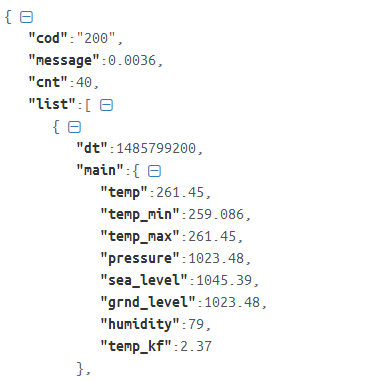
\includegraphics[width=0.8\textwidth]{Bild1}
\caption{Registry laufen lassen}
\end{center}
\end{figure}

Jetzt öffnet man eine weiter Eingabeaufforderung und lässt den Server mit dem Befehl \textit{java ChatServerImpl} laufen. Anschließend öffnet man beliebig viele weitere Eingabeaufforderungen, wo man dann die einzelnen Clients erstellen kann. Nun kann man mit mehreren Clients kommunizieren und sich am Ende mit \textit{.LOGOUT} "ausloggen" (siehe Abbildung 2).  \\
\\

\begin{figure}[htbp]
\begin{center}
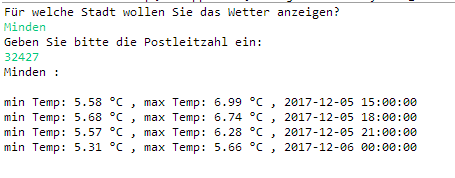
\includegraphics[width=0.8\textwidth]{Bild2}
\caption{Kommunikation mit mehreren Clients}
\end{center}
\end{figure}

\subsection{Ergebnis}
Es ist uns möglich ein einfaches Chat-System mit der Java RMI zu erstellen und dieses auch anzuwenden.

\section{Quellen}
\begin{thebibliography}{999}

\bibitem {1} Nifal Nizar, SMTP - RMI Multiple Clients Chat Program \\ \url{https://easycodestuff.blogspot.de/2014/11/rmi-chat-program-using-java.html}, 27.11.2017

\bibitem {2} Oracle, Trail: RMI \\ \url{https://docs.oracle.com/javase/tutorial/rmi/index.html}, 27.11.2017

\bibitem {3} Kobi Ianko, java.rmi.UnknownHostException \\ \url{https://developer.jboss.org/thread/152290?_sscc=t}, 27.11.2017

\end{thebibliography}
